\section{描述性统计}
\sectionlead{section-3}{三、描述性统计}{研究深度、主题分布与价格回看窗口}

\subsection{3.1 研究投入}
\begin{frame}[label=funnel]{两层样本回答不同的研究投入问题}
  \crumb{Part 3}{3.1 研究投入}{II.A、II.C · Table 2}
  \begin{columns}[T,onlytextwidth]
    \column{.59\textwidth}\centering
    \begin{tikzpicture}[x=1cm,y=.81cm,font=\small]
      \foreach \y/\width/\shade/\layertext in {
        4/3.16/8/{数万户 · 约 20 亿条 URL},
        3/2.95/13/{\textcolor{sampleblue}{\textbf{484 户}} · 约 850 万条点击},
        2/2.74/18/{约 \textbf{3,000 小时}研究},
        1/2.53/23/{约 \textbf{1,350 小时}匹配标的},
        0/2.32/28/{\textcolor{samplegold}{\textbf{50 户}} · 高代码匹配子样本}} {
        \path[fill=wine!\shade] (-\width,\y+.45)--(\width,\y+.45)--
          ({\width-.17},\y-.45)--({-\width+.17},\y-.45)--cycle;
        \node at (0,\y) {\layertext};
      }
    \end{tikzpicture}\par
    {\scriptsize 形状示意处理顺序与子样本，宽度无数量刻度。}
    \column{.39\textwidth}\small
    \textcolor{sampleblue}{\textbf{484 户 · 总体投入}}\par
    估计研究总量与主题分布，不要求每条研究链接都匹配个股。\par\medskip
    \textcolor{samplegold}{\textbf{50 户 · 高代码匹配}}\par
    研究 URL 大多能直接或经相邻记录匹配股票代码，可限定到所交易股票。
  \end{columns}
  \finding{后文并列总体与高匹配子样本。50 户按研究链接的代码匹配质量选取，并非只有这 50 户能识别订单。}
\end{frame}

\begin{frame}[label=categories]{研究内容与混合页面的归类}
  \crumb{Part 3}{3.1 研究投入 · 内容分类}{II.C · Table 3 · Table IA2}
  \small
  \textbf{11 类内容}\par\smallskip
  \begin{tabularx}{\linewidth}{@{}YY@{}}
    风险统计、盈利、股利 & 其他基本面、分析师、知情持股\\
    价格图、技术信号 & 公司官网、其他、未确定\\
  \end{tabularx}\par\medskip
  \textbf{3 种混合格式：一页可以包含多个主题}\par\smallskip
  \begin{tabularx}{\linewidth}{@{}L{.27\linewidth}Y@{}}
    \toprule 页面格式 & 时间如何分到具体主题\\\midrule
    综合行情快照 & 正文按各主题专门页面的参与比例分配（兴趣权重）。\\
    未确定类型的新闻 & 依据 RavenPack 新闻内容分类的分布分配。\\
    留言板 & 依据 Reddit r/stocks 帖子主题的分布分配。\\\bottomrule
  \end{tabularx}
  \finding{按信息内容分类；快照、新闻与留言板先保留格式，再报告分配后的主题时间。}
\end{frame}

\newcommand{\depthbars}[5]{%
  \node[anchor=east] at (0,#1+.26) {#2};
  \fill[#3!38] (0,#1+.28) rectangle (#4,#1+.53);
  \fill[#3] (0,#1-.02) rectangle (#5,#1+.23);
  \node[anchor=west,text=#3] at (#4,#1+.40) {#4};
  \node[anchor=west,text=#3,font=\small\bfseries] at (#5,#1+.09) {#5};}
\begin{frame}[label=depth]{每笔研究分钟，先在户内计算}
  \crumb{Part 3}{3.1 研究投入}{Table 2 B/C}
  \[
    r_i(S)=\frac{\text{投资者 }i\text{ 在 }S\text{ 的研究分钟}}{\text{投资者 }i\text{ 的订单笔数}},
    \qquad \overline r_S=\frac{\sum_i r_i(S)}{N},\quad \operatorname{Med}_i r_i(S).
  \]
  {\small \(i\)：投资者（家庭）；\(S\)：统计的股票范围。先按户计算，再跨户汇总。}
  {\centering
  \begin{tikzpicture}[x=.046cm,y=.72cm,font=\small]
    \depthbars{2}{484 户 · 全部股票}{sampleblue}{144.2}{36.4}
    \depthbars{1}{50 户 · 全部股票}{samplegold}{96.8}{51.7}
    \depthbars{0}{50 户 · 所交易股票}{samplegold}{29.1}{5.7}
    \node[anchor=west] at (0,-.39) {分钟／笔 \quad 浅色均值 \quad 深色中位数};
  \end{tikzpicture}\par}
  \finding{同一 50 户：限定到交易标的，中位数由 51.7 降至 5.7 分钟。全部研究还含未交易股票及部分难配码记录。\textbf{均值远高于中位数，投入呈右偏长尾。}}
  \scriptsize\jump{appendix-5}{A5 · 画像与时长原表}
\end{frame}

\newcommand{\profilebars}[4]{%
  \node[anchor=west,font=\scriptsize\bfseries] at (0,#1+.92) {#2};
  \fill[sampleblue!37] (0,#1+.32) rectangle (1,#1+.58);
  \fill[sampleblue] (0,#1-.02) rectangle ({#4/#3},#1+.24);
  \node[anchor=west,inner sep=2pt] at (1,#1+.45) {#3};
  \node[anchor=west,inner sep=2pt] at ({#4/#3},#1+.11) {#4};}
\begin{frame}[label=domains]{典型家庭交易不多，研究横跨多个站点}
  \crumb{Part 3}{3.1 研究投入}{Table 1 · Table 2 B}
  \pair{\small\textbf{样本画像 · 484 户}\par
    \begin{tikzpicture}[x=3.05cm,y=.42cm,font=\scriptsize]
      \profilebars{3.2}{股票交易 · 笔／月}{2.2}{0.7}
      \profilebars{1.6}{券商浏览 · 分钟／月}{214.2}{81.6}
      \profilebars{0}{交易金额 · 千美元／笔}{13.5}{2.0}
    \end{tikzpicture}\par
    {\scriptsize 每组内部同比例。浅为均值，深为中位数；金额按 191 户。}}
  {\small\textbf{每笔研究时间 · 484 户均值}\par
    \begin{tabularx}{\linewidth}{@{}Yr@{}}\toprule
    浏览来源 & 分钟／笔\\\midrule
    券商 & 55.7\\
    Yahoo Finance & 45.3\\
    其他财经网站 & 41.9\\
    公司官网 & 1.3\\\bottomrule
    \end{tabularx}}
  \medskip
  \begin{center}
  \begin{tikzpicture}[x=.068cm,y=.62cm,font=\small]
    \fill[sampleblue!57] (0,0) rectangle (55.7,.7);
    \fill[sampleblue!35] (55.7,0) rectangle (101,.7);
    \fill[samplegold!43] (101,0) rectangle (142.9,.7);
    \fill[samplegold] (142.9,0) rectangle (144.2,.7);
    \node at (27,.35) {券商};
    \node at (78,.35) {Yahoo};
    \node at (122,.35) {其他财经};
  \end{tikzpicture}
  \end{center}
  \finding{一共 144.2 分钟／笔，按均值加总，约 61\% 发生在券商站外。}
\end{frame}

\subsection{3.2 主题与窗口}
\newcommand{\topicbars}[4]{%
  \node[anchor=east] at (0,#1) {#2};
  \fill[sampleblue!60] (0,#1-.17) rectangle (#3*.031,#1+.17);
  \node[anchor=west,inner sep=2pt] at (#3*.031,#1) {#3\%};
  \fill[samplegold!68] (4.38,#1-.17) rectangle (4.38+#4*.064,#1+.17);
  \node[anchor=west,inner sep=2pt] at (4.38+#4*.064,#1) {#4};}
\begin{frame}[label=topics]{价格图的参与范围和平均用时都居前}
  \crumb{Part 3}{3.2 主题与窗口}{Table 3 · 484 户，全部股票}
  \begin{center}
    \begin{tikzpicture}[x=1.06cm,y=.56cm,font=\small]
      \node[anchor=west,text=sampleblue,font=\small\bfseries] at (0,6.9) {参与家庭比例};
      \node[anchor=west,text=samplegold,font=\small\bfseries] at (4.38,6.9) {均值分钟／交易};
      \topicbars{6}{价格图}{93}{39.1}
      \topicbars{5}{综合行情}{93}{37.0}
      \topicbars{4}{分析师资料}{71}{12.5}
      \topicbars{3}{其他基本面}{53}{2.6}
      \topicbars{2}{盈利}{40}{1.7}
      \topicbars{1}{股利}{17}{0.6}
      \topicbars{0}{风险统计}{1}{0.0}
    \end{tikzpicture}
  \end{center}
  \finding{两列分别读“多少家庭看过”和“平均花多少时间”。图为直接分类的代表性项目；约 1\% 的风险统计覆盖对应 7 户。}
  \scriptsize\jump{appendix-1}{A1 · 主题原表}
\end{frame}

\begin{frame}[t,label=mixed]{综合行情的混合内容如何分到主题}
  \crumb{Part 3}{3.2 主题与窗口}{Table 3 · Table IA2}
  \begin{columns}[T,onlytextwidth]
  \column{.53\textwidth}\small
    \textbf{AAPL 综合行情页 · 当代实例}\par\smallskip
    \begingroup\setlength{\parskip}{0pt}
    {\setlength{\fboxsep}{1pt}\color{wine}\fbox{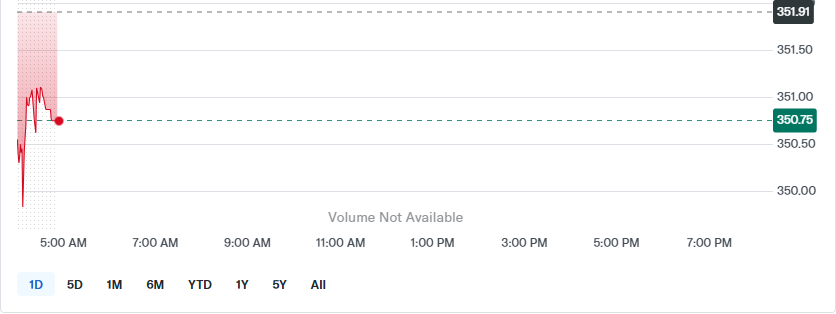
\includegraphics[width=.86\linewidth]{yahoo-chart.png}}}\par
    {\setlength{\fboxsep}{1pt}\color{sampleteal}\fbox{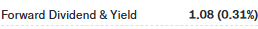
\includegraphics[width=.86\linewidth]{yahoo-dividend.png}}}\par
    {\setlength{\fboxsep}{1pt}\color{sampleteal}\fbox{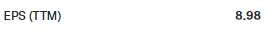
\includegraphics[width=.86\linewidth]{yahoo-eps.png}}}\par
    {\scriptsize Yahoo Finance · 2026-11-18 · 同页裁剪}\par\endgroup
  \column{.44\textwidth}
    \textbf{价格图的均值分钟／笔}\par
    \greatnum{39.1}\enspace\(\to\)\enspace\greatnum{64.4}\par
    {\small 直接分类 \hfill 兴趣权重插补}\par\smallskip
    {\small\textbf{视觉权重（备选）}\par
    按不同内容占据的展示行数分配。\par\smallskip
    \textbf{兴趣权重（正文）}\par
    按各主题专门页面的参与比例分配。}
  \end{columns}
  \finding{\textcolor{wine}{价格图}与\textcolor{sampleteal}{EPS、股利等}同页出现。混合页分配后，价格图仍居首；64.4 使用兴趣权重。}
  \small\jump{appendix-3}{A3 · 权重细节}
\end{frame}

\begin{frame}[label=windows]{含默认图时日内占主，主动调整多看数月}
  \crumb{Part 3}{3.2 主题与窗口}{Figure 1 A/B · 484 户}
  \pair{\small\textbf{A · 全部图表访问}\par
    \annotatedpanel{3.80cm}{fig1a.pdf}{\draw[wine,line width=.65pt] (.14,.13) rectangle (.183,.93);}\par
    {\small 约 73\% 是默认的 1 日窗口。}}
  {\small\textbf{B · 只看主动调整}\par
    \annotatedpanel{3.80cm}{fig1b.pdf}{\draw[wine,line width=.65pt] (.35,.13) rectangle (.66,.98);}\par
    {\small 3 个月和 1 年是明显峰值。}}
  \finding{默认日内图之外，主动调整者多看数月到一年。两图均为各自面板内的访问次数占比。}
\end{frame}

\begin{frame}[label=averages]{描述性事实与模型的信息输入}
  \crumb{Part 3}{小结与衔接}{Tables 2--3 · Figure 1 · 输入假设的比较}
  \footnotesize
  \setlength{\tabcolsep}{3pt}
  \renewcommand{\arraystretch}{1.06}
  \begin{tabularx}{\linewidth}{@{}L{.26\linewidth}L{.18\linewidth}Y@{}}
    \toprule 理论／信息假设 & 现有事实的关系 & 证据逻辑\\\midrule
    组合选择的风险输入 & 较不一致 & 主动查看风险统计约 1\%，显式风险量很少被调取。\\
    DSSW 噪声交易 & 部分一致 & 研究较薄且偏价格；无法直接判断信息价值。\\
    Hong--Stein & 待第四部分 & 需看不同投资者怎样组合新闻和价格。\\
    BSV 盈利信号 & 部分一致 & 盈利覆盖 40\%，直接投入较短。\\
    收益外推 & 输入一致 & 价格图覆盖 93\%，主动窗口常为数月到一年。\\
    股利信号 & 证据有限 & 股利覆盖 17\%，直接研究较少。\\
    有限注意力 & 待第四部分 & 需看财报与事件是否吸引集中关注。\\
    同质信息输入 & 较不一致 & 均值明显高于中位数，投入差异很大。\\
    \bottomrule
  \end{tabularx}
  \smallskip
  {\small 均值／中位数：全样本全部股票 \textbf{144.2／36.4}；50 户交易标的 \textbf{29.1／5.7} 分钟／笔。}
\end{frame}
